The test is almost complete -- the only step remaining is to ''map'' your specification to the \gdaut{}. 

Object mapping involves two steps: collecting details about the objects you want to test from the 
\gdaut{},  and assigning them to the component names you defined in the \gdsteps{}. 

\begin{enumerate}
\item In the \gdtestsuitebrowser{}, right-click on the node for the \bxname{SimpleAdderTest} and select:\\
\bxmenu{Open with}{\jb{} object mapping editor}{}
\item When the editor appears, click the \bxcaption{Start the mapping mode} button on the toolbar.  
\item Activate the \gdaut{} by clicking in its title bar. 
\item Move the mouse over objects in the \gdaut{}. You will see that supported components are highlighted with a green border when the cursor moves over them (\bxfigref{TutGreenBorders}).

 \begin{figure}[h]
\begin{center}
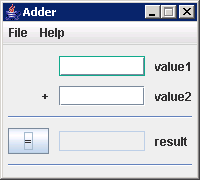
\includegraphics{Tasks/Objectmapping/PS/greenborders}
\caption{Green borders around supported component}
\label{TutGreenBorders}
\end{center}
\end{figure}

\item Hover the cursor over the \bxcaption{value1} text input field 
(just left of the \bxcaption{value1} label) and press
\bxkey{Ctrl+Shift+A}. 
\item If you look in the \gdomeditor{}, you will see that the name and details for this component have been ''collected'' (\bxfigref{TutCollectName1}).
\begin{figure}[h]
\begin{center}
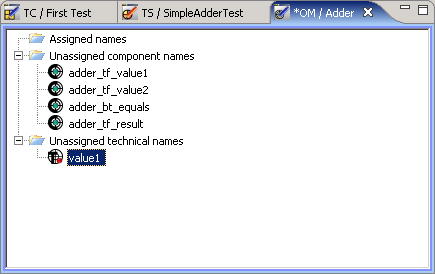
\includegraphics{Tutorials/PS/TutCollectName1}
\caption{Collected technical name}
\label{TutCollectName1}
\end{center}
\end{figure}

 
\item Repeat the step to map \bxcaption{value2} field, the equals button and the \bxcaption{result} field,
respectively.
\item In the \gdomeditor{}, assign your component name for the first text input field (\bxcaption{adder\_tf\_value1}) to the name for this field that you mapped from the \gdaut{}. You assign names by dragging and dropping the component names to the technical names (the names from the \gdaut{}).
\item Repeat this step for the other component and technical names (\bxfigref{TutOM}).
\begin{figure}[h]
\begin{center}
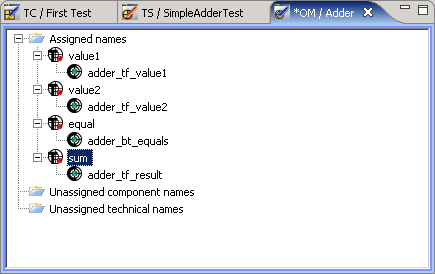
\includegraphics{Tutorials/PS/TutOM}
\caption{Completed object mapping}
\label{TutOM}
\end{center}
\end{figure}
 
\item Press the \bxcaption{stop \gdomm{} button} and then \bxcaption{save}. 
\end{enumerate}




